\chapter{%
    O Comportamento \glsentrytext{pressure}, \glsentrytext{specificVolume},
    \glsentrytext{temperature} das Substâncias Puras
}
\label{chap:pureSubstances}

    Afirmamos no início que o estado (de equilíbrio) de um sistema deve ser
    estabelecido pelo valor (instantâneo) de suas propriedades. A pergunta
    natural que deveria nos ocorrer é: no mínimo quantas --- e quais --- as
    propriedades termodinâmicas que são necessárias para se fixar o estado do
    sistema?  Existe alguma relação de dependência entre elas, ou seriam elas
    todas independentes entre si, ou seja, poderiam ser alteradas
    independentemente?


    \section{Sistema Compressível Simples}

    Bem, embora não tenhamos uma resposta definitiva que se aplique a qualquer
    sistema termodinâmico em geral, um importante postulado virá em nosso
    socorro. Mas antes precisamos definir o sistema compressível simples. Este
    é o sistema especial para o qual os únicos trabalhos mecânicos relevantes
    são o de expansão e compressão da fronteira do tipo
    \gls{pressure}\diff{\gls{volume}} além de um possível trabalho de
    cisalhamento, o trabalho de eixo, que atravessa a sua fronteira. Essa
    condição, não por coincidência, representa a nossa ênfase em sistemas de
    potência e refrigeração, ou engenharia de energia.


    \section{O Postulado dos Estados}

    Podemos afirmar que para um sistema compressível simples (composto de uma
    única substância pura), o estado termodinâmico será definido pelo valor de
    duas propriedades intensivas independentes além da extensão do referido
    sistema. Este é o chamado Postulado dos Estados e possui uma imensa
    importância prática, pois nos permite afirmar que o estado intensivo de um
    sistema compressível simples (uma substância pura) pode ser representado
    por um par não ordenado construído com os valores de duas propriedades
    termodinâmicas intensivas independentes, como por exemplo
    $(\gls{temperature},\gls{specificVolume})$ ou
    $(\gls{pressure},\gls{temperature})$.

    A extensão do sistema a que o Postulado dos Estados se refere será dada
    direta ou indiretamente por qualquer uma das massas que compõem o sistema.

    De fato, graças a nossa definição de propriedade termodinâmica extensiva
    como sendo linear com a massa, podemos adotar como princípio que qualquer
    uma das massas envolvidas no problema que estamos modelando poderá exercer
    o papel de fator de escala para aquele problema.

    A massa poderá sempre ser utilizada como um fator de escala. Portanto,
    qualquer problema de Termodinâmica sempre poderá ser descrito em termos de
    propriedades intensivas e \enquote{intensivadas}, bastando para isso se
    dividirem as equações por qualquer uma das massas envolvidas no problema.

    Por causa do Postulado dos Estados, se selecionarmos quaisquer duas
    propriedades intensivas ou \enquote{intensivadas} independentes entre si de
    uma substância pura para compor os eixos de um sistema de coordenadas
    retangulares, todas as demais propriedades intensivas ou
    \enquote{intensivadas} serão necessariamente dependentes e terão seus
    valores sobre o terceiro eixo determinados de alguma forma, gerando assim
    um espaço tridimensional de estados para cada uma das propriedades
    dependentes.

    Portanto, para uma substância pura, as propriedades \gls{pressure},
    \gls{specificVolume}, \gls{temperature} não podem ser todas independentes
    ao mesmo tempo.

    Mas como se comporta um substância pura do ponto de vista de suas
    propriedades \gls{pressure}, \gls{specificVolume}, \gls{temperature}? Vamos
    começar com a água, devido a nossa experiência cotidiana com ela.


    \section{O Comportamento da Água}

    Imagine uma panela com água pura à pressão atmosférica ao nível do mar de
    \SI{101.32}{\kilo\pascal} ou \SI{1}{atm} (o que é a pressão atmosférica?) e
    à temperatura de \SI{25}{\celsius}. Note que, pelo que já aprendemos a
    respeito de sistemas compressíveis simples, uma vez que duas propriedades
    intensivas independentes são fornecidas, o estado termodinâmico intensivo
    está definido. Sabemos pela nossa experiência científica cotidiana que
    neste estado a água se encontra na fase líquida, na região chamada de
    líquido comprimido. Vamos então, enquanto mantendo a pressão constante,
    aquecer lentamente, isto é, fornecer calor, à água. A temperatura da água
    vai aumentando e, portanto, altera-se o seu estado. O que acontece com o
    volume específico (que é o inverso da densidade)?  Entretanto, sabemos da
    experiência que a temperatura não aumenta indefinidamente! Ao chegar aos
    \SI{100}{\celsius} nesta pressão, surge a primeira bolha de vapor de água -
    inodoro, insípido e incolor  e com um volume específico muito maior do que
    o líquido de onde se originou. É o ponto de líquido saturado. Se
    continuarmos com o fornecimento de calor, notaremos que a temperatura
    estacionará nos \SI{100}{\celsius} e o vapor irá se tornando mais e mais
    abundante. A temperatura se torna uma função de \gls{pressure},
    \gls{satTemperature}\functionOf{\gls{pressure}}. Esta é a região de
    saturação, dentro da qual existe uma mistura heterogênea de proporções
    variáveis de ambas as fases: a fase de liquido saturado e a fase de vapor
    saturado. Exatamente quando a fase de líquido saturado deixa de existir,
    este é o ponto de vapor saturado ou vapor saturado seco. Se prosseguirmos
    com o fornecimento de calor, a temperatura voltará a aumentar e obteremos
    um vapor cada vez mais quente. Esta é a região de vapor superaquecido.
    Vejamos na \cref{fig:diagramTvPureSubstance} este comportamento em um
    plano de \gls{temperature}, \gls{specificVolume} mantendo-se \gls{pressure}
    constante.

    Na região de líquido comprimido, em que a temperatura \gls{temperature} é
    menor do que a temperatura de saturação \gls{satTemperature} dada
    pela pressão \gls{pressure}, $\gls{temperature} <
    \gls{satTemperature}\functionOf{\gls{pressure}}$, o volume
    específico
    \gls{specificVolume}\functionOf{\gls{pressure},\gls{temperature}} varia
    muito pouco com a pressão, o que era de se esperar, pois o líquido (como os
    sólidos) é muito pouco compressível.

    Na região de saturação, em que a temperatura é exatamente igual a
    \gls{satTemperature}\functionOf{\gls{pressure}}, o sistema água torna-se,
    como já dissemos, uma mistura heterogênea e passa a ser composto de dois
    subsistemas: o líquido saturado, com volume específico
    \gsub{specificVolume}{satLiquid}\functionOf{\gls{pressure}} e o vapor
    saturado, com volume específico
    \gsub{specificVolume}{satVapor}\functionOf{\gls{pressure}}. Observe que
    para a determinação do volume específico do líquido saturado e do volume
    específico do vapor saturado basta conhecermos a temperatura
    \gls{satTemperature}\functionOf{\gls{pressure}} ou então a pressão
    \gls{pressure}.

    \begin{figure}[!htb]
        \caption{%
            A saturação líquido-vapor na projeção
            \gls{temperature}-\gls{specificVolume}
        }

        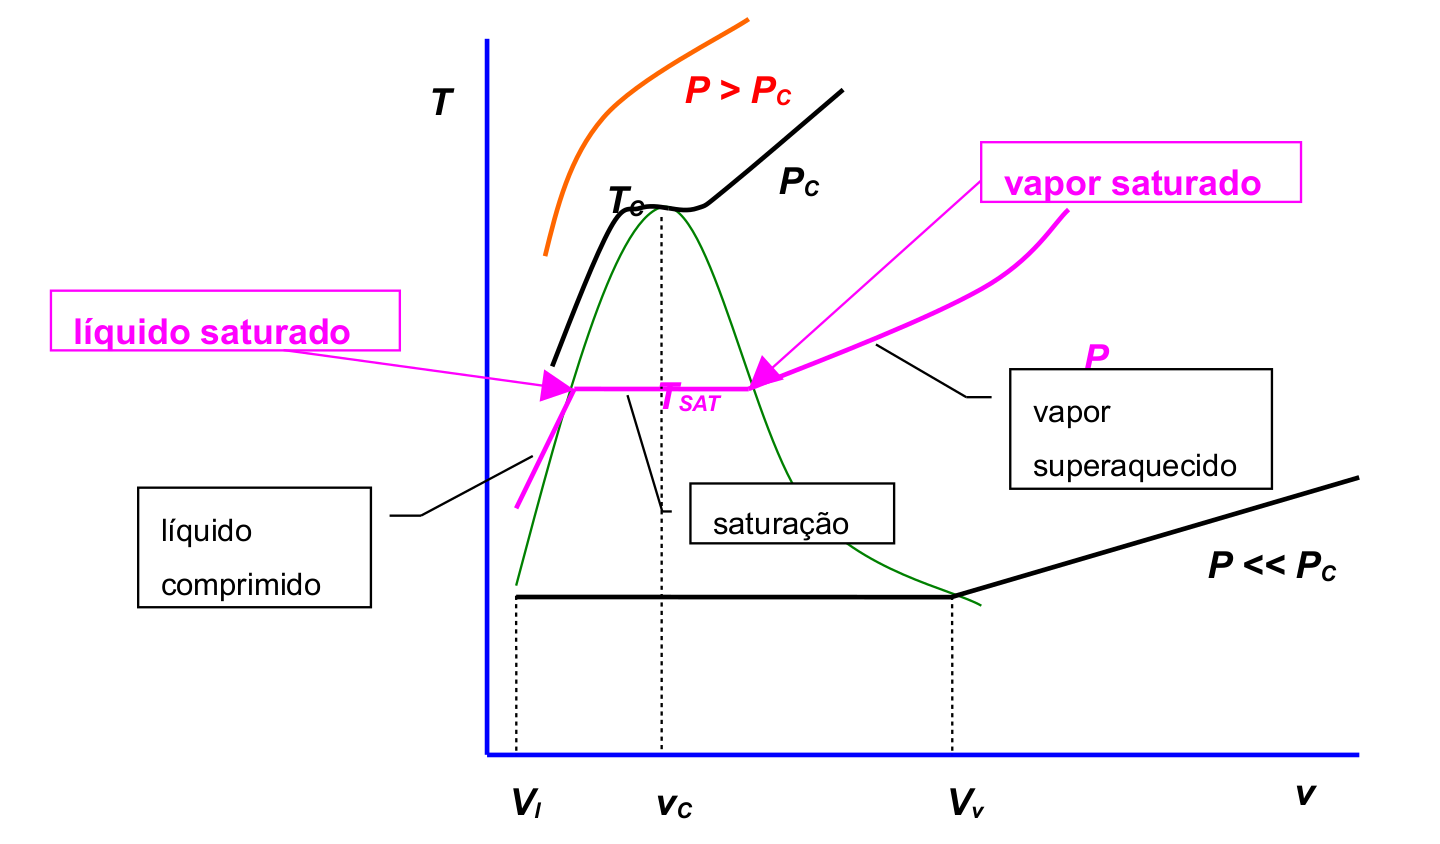
\includegraphics[
            width=\textwidth
        ]   {diagramTvPureSubstance.png}

        \label{fig:diagramTvPureSubstance}
    \end{figure}

    Como o sistema pode ser composto desde praticamente muito líquido saturado
    e pouco vapor saturado até muito vapor saturado e pouco líquido saturado,
    passando por todos os estados intermediários, é interessante que seja
    definida uma nova grandeza para representar esta distribuição. Seja
    \gls{mass} a massa invariante do sistema e \gls{volume} o seu volume total.
    A massa e o volume da fase líquida serão \gsub{mass}{satLiquid},
    \gsub{volume}{satLiquid} e para a fase vapor serão \gsub{mass}{satVapor},
    \gsub{volume}{satVapor} respectivamente.  Podemos então expressar o volume
    o volume e a massa totais da mistura pelas \cref{eq:satMixtureProps}.
    %
    \begin{subequations}
        \label{eq:satMixtureProps}

        \begin{equation} \label{eq:satTotalVolume}
            \gls{volume}
            =
            \gsub{volume}{satLiquid}
            +
            \gsub{volume}{satVapor}
        \end{equation}
        \begin{equation} \label{eq:satTotalMass}
            \gls{mass}
            =
            \gsub{mass}{satLiquid}
            +
            \gsub{mass}{satVapor}
        \end{equation}
    \end{subequations}
    %
    e, portanto,
	%
	\begin{equation} \label{eq:1.2}
        \gls{mass}
        \gls{specificVolume}
        =
        \gsub{mass}{satLiquid}
        \gsub{specificVolume}{satLiquid}
        \functionOf{
            \gls{pressure}
        }
        +
        \gsub{mass}{satVapor}
        \gsub{specificVolume}{satVapor}
        \functionOf{
            \gls{pressure}
        }
    \end{equation}

    Se definirmos o título do vapor \gls{vaporQuality} como $\gls{vaporQuality}
    = \dfrac{\gsub{mass}{satVapor}}{\gls{mass}}$  então o volume específico da
    mistura toda \gls{specificVolume} será (prove isso...):
	%
	\begin{equation} \label{eq:1.3}
        \gls{specificVolume}
        \functionOf{
            \gls{pressure},
            \gls{vaporQuality}
        }
        =
        (1 - \gls{vaporQuality})
        \gsub{specificVolume}{satLiquid}
        \functionOf{
            \gls{pressure}
        }
        +
        \gls{vaporQuality}
        \gsub{specificVolume}{satVapor}
        \functionOf{
            \gls{pressure}
        }\,.
    \end{equation}

    Como o título, %
    % $\mathit{mv}=m_lv_l(P)+m_vv_v(P)$ Is this correct here or it a typo?
    \gls{vaporQuality}, foi definido a partir de uma combinação de propriedades
    termodinâmicas, é por sua vez uma propriedade termodinâmica (você acha que
    é intensiva ou extensiva?).  Portanto, o estado intensivo da mistura
    heterogênea estará completamente estabelecido pela pressão (ou pela
    temperatura) e pelo título \gls{vaporQuality}. Você consegue determinar  os
    valores de \gls{vaporQuality} para líquido saturado e vapor saturado?  Como
    seria uma linha de \gls{vaporQuality} constante na
    \cref{fig:diagramTvPureSubstance}?

    Se realizarmos o experimento a pressões \gls{pressure} superiores,
    percebemos que \gls{satTemperature}\functionOf{\gls{pressure}} aumentará e
    a pressões menores, \gls{satTemperature}\functionOf{\gls{pressure}} se
    reduzirá. Pode explicar então porque é melhor cozinhar utilizando a panela
    de pressão? O lugar geométrico de todos os pontos de líquido saturado e de
    vapor saturado configura o domo de vapor, que abrange toda a região de
    saturação.

    A significativa diferença entre \gsub{specificVolume}{satVapor} e
    \gsub{specificVolume}{satLiquid} diminui a medida em que aumentamos a
    temperatura (ou a pressão) até que a diferença se reduzirá a um único ponto
    (\gsub{specificVolume}{critical}) no ponto crítico. No ponto crítico a
    temperatura é \gsub{temperature}{critical} e a pressão será
    \gsub{pressure}{critical}. Na região definida pela pressão
    \gsub{pressure}{critical} e acima dela a mistura heterogênea deixa de
    existir e é denominada região supercrítica. Observe que, exatamente no
    ponto crítico, a curva de pressão crítica possui um ponto de inflexão (o
    que é isso?) e é a única curva de pressão que tem esta característica. Para
    qualquer temperatura, quando a pressão é maior ou igual a PC não existe
    mais distinção entre gás e líquido (trata-se de uma única fase muito
    densa).

    Na região de vapor superaquecido, em que a temperatura \gls{temperature} é
    maior do que \gls{satTemperature}\functionOf{\gls{pressure}} na pressão
    \gls{pressure},
    $\gls{temperature}>\gls{satTemperature}\functionOf{\gls{pressure}}$, o
    volume específico
    \gls{specificVolume}\functionOf{\gls{pressure},\gls{temperature}} varia
    bastante com a temperatura, uma característica da compressibilidade dos
    gases e vapores. Por outro lado, quando a pressão \gls{pressure} é muito
    menor do que \gsub{pressure}{critical} a curva de pressão constante na
    região de vapor superaquecido torna-se praticamente uma reta e o gás
    torna-se pouco denso.  Esta é a região do gás perfeito (ou ideal), na qual,
    quando a pressão (que é muito baixa) é constante, o volume do gás é
    diretamente proporcional à sua temperatura.

    Acabamos de analisar o comportamento da água através da variação da
    temperatura enquanto mantemos a pressão \gls{pressure} constante.

    Vejamos então o que acontece no plano \gls{pressure},\gls{specificVolume}
    enquanto se varia a pressão mantendo-se \gls{temperature} constante, como
    representado na \cref{fig:diagraPvPureSubstance}.

    Consideremos a água agora a uma pressão inicial \gls{pressure} elevada,
    como \SI{40}{\mega\pascal}, e à temperatura sempre fixa de
    \SI{100}{\celsius}, ou seja, como líquido comprimido (pois
    $\gls{pressure}>\gls{satPressure}\functionOf{\gls{temperature}}$.
    Fornecendo calor, vamos diminuir a pressão, enquanto mantemos a temperatura
    \gls{temperature} inalterada. A partir de água encerrada em um conjunto
    cilindro-pistão, você consegue conceber um experimento que possa realizar
    este processo? Quando alcançarmos a pressão de \SI{101.325}{\kilo\pascal}
    (ou \SI{1}{atm}), surgirá a primeira bolha de vapor: já sabemos, é o ponto
    de líquido saturado,
    \gsub{specificVolume}{satLiquid}\functionOf{\gls{temperature}}. Se
    continuarmos o processo (como?), a pressão
    \gls{satPressure}\functionOf{\gls{temperature}} permanecerá constante, ao
    passo que a quantidade de vapor saturado irá aumentando: esta é a já nossa
    conhecida região de saturação, que, como você sabe, é uma mistura de
    líquido saturado e vapor saturado.

    Quando a última gota de líquido saturado converter-se em vapor saturado,
    que é o ponto de vapor saturado,
    \gsub{specificVolume}{satVapor}\functionOf{\gls{temperature}}, a pressão
    poderá voltar a cair outra vez e estaremos na região de vapor
    superaquecido, em que
    $\gls{pressure} > \gls{satPressure}\functionOf{\gls{temperature}}$ e
    \gls{specificVolume}\functionOf{\gls{pressure},\gls{temperature}}.

    Se a pressão continuar caindo, chegaremos a uma região ($\gls{pressure} \ll
    \gsub{pressure}{critical}$) em que a pressão e o volume específico
    assumirão um caráter hiperbólico, do tipo
    $\gls{pressure}\gls{specificVolume} = constante$. O que você conclui sobre
    essa região?

    Se realizarmos o experimento a temperaturas \gls{temperature} superiores,
    percebemos que \gls{satPressure}\functionOf{\gls{temperature}} aumentará e
    a temperaturas menores, \gls{satPressure}\functionOf{\gls{temperature}} se
    reduzirá. Novamente, o lugar geométrico de todos os pontos de liquido
    saturado \gsub{specificVolume}{satLiquid}\functionOf{\gls{temperature}} e
    de vapor saturado
    \gsub{specificVolume}{satVapor}\functionOf{\gls{temperature}} configura o
    domo de vapor, que abrange toda a região de saturação.

    \begin{figure}[!htb]
        \caption{%
            A saturação líquido-vapor na projeção
            \gls{pressure}-\gls{specificVolume}
        }

        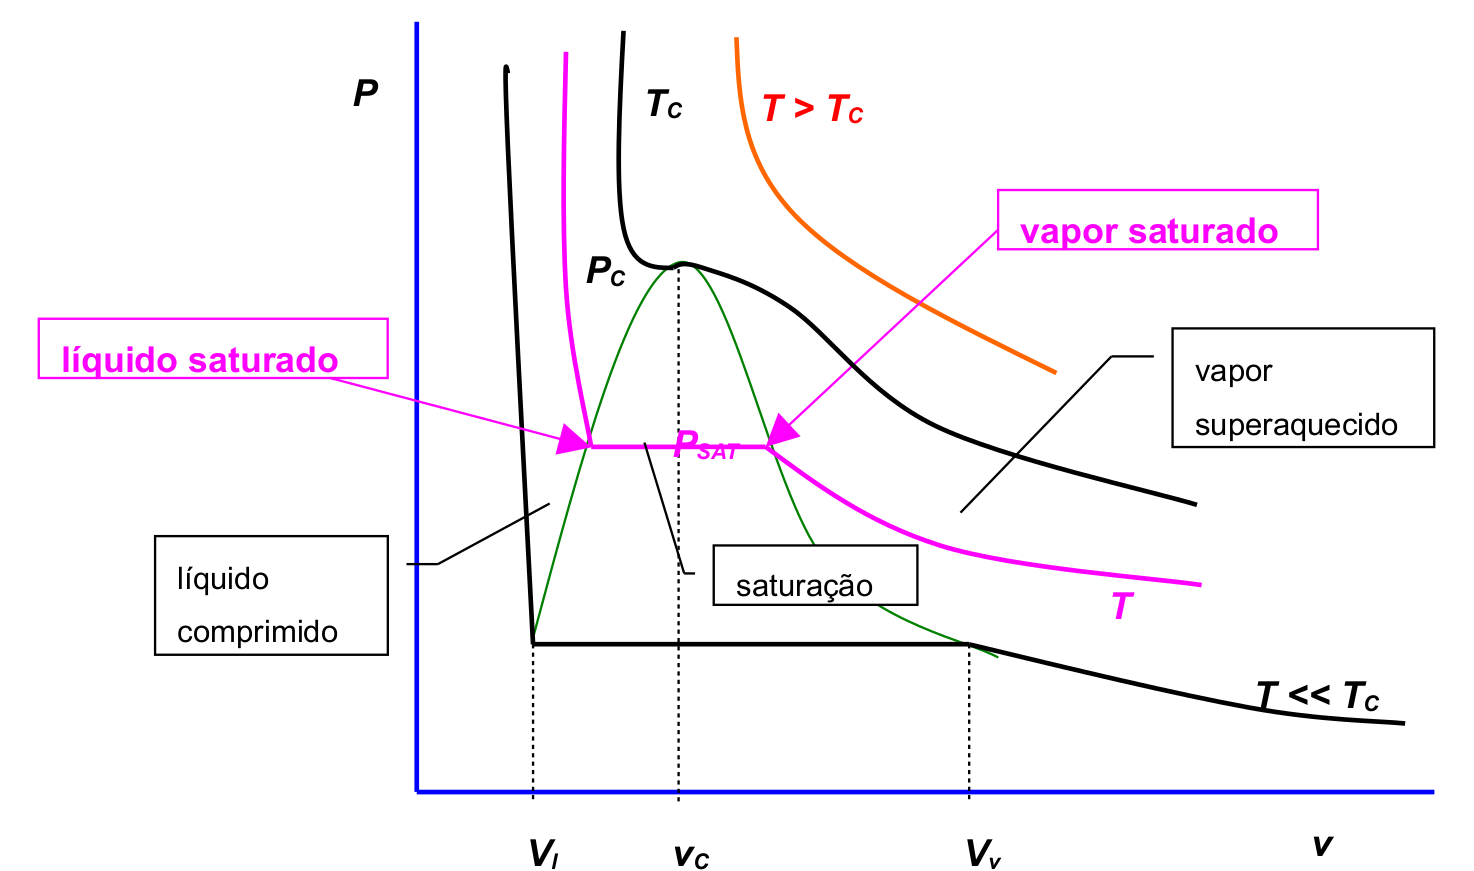
\includegraphics[
            width=\textwidth
        ]   {diagramPvPureSubstance.png}

        \label{fig:diagraPvPureSubstance}
    \end{figure}

    A significativa diferença entre
    \gsub{specificVolume}{satVapor}\functionOf{\gls{temperature}} e
    \gsub{specificVolume}{satLiquid}\functionOf{\gls{temperature}} diminui a
    medida em que aumentamos a temperatura (ou a pressão) até que a diferença
    se reduzirá a um único ponto $(\gsub{specificVolume}{critical})$ no ponto
    crítico. No ponto crítico a pressão é \gsub{pressure}{critical} e à
    temperatura \gsub{temperature}{critical} e acima dela a região de saturação
    deixa de existir.  Observe que, exatamente no ponto crítico, a curva de
    temperatura crítica possui um ponto de inflexão (o que é isso?) e é a única
    curva de temperatura que tem esta característica. Para qualquer pressão,
    quando a temperatura é maior do que \gsub{temperature}{critical} não existe
    mais distinção entre gás e líquido (trata-se de uma única fase muito
    densa). Você adivinhou, esta é a região supercrítica.

    Vejamos o que acontece com a água no plano \gls{pressure},\gls{temperature}
    enquanto mantemos \gls{specificVolume} constante, conforme mostrado na
    \cref{fig:diagramPTWater}. Na figura observamos as três fases principais
    para a água: gás, líquido e sólido. Aprendemos anteriormente que na
    saturação, o processo a pressão constante se dá também a temperatura
    constante, ao passo que o processo a temperatura constante se dá também a
    pressão constante (sabe dizer por quê?). Então as regiões de saturação,
    como o domo de vapor, devem ser reproduzidas no plano \gls{pressure},
    \gls{temperature} como linhas curvas, as chamadas superfícies planas.

    \begin{figure}[!htb]
        \caption{%
            Comportamento no plano \gls{pressure}-\gls{temperature} da água
        }

        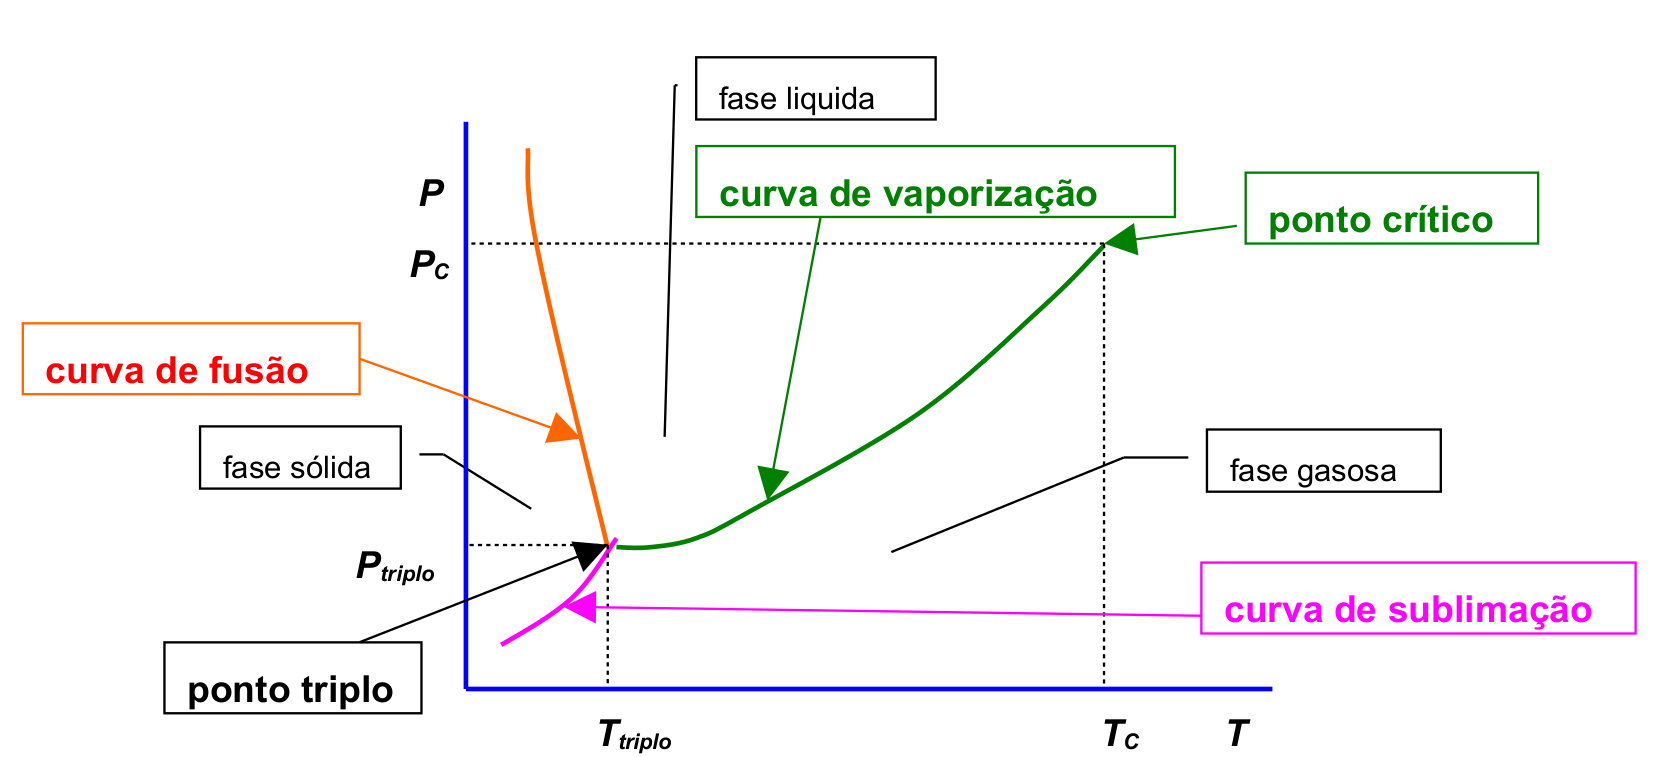
\includegraphics[
            width=0.70\textwidth
        ]   {diagramPTWater.png}

        \label{fig:diagramPTWater}
    \end{figure}

    Já conhecíamos a região líquido-vapor da qual se origina a curva de
    vaporização (ou curva de pressão de vapor). Note o ponto crítico:
    $\gsub{temperature}{critical},\gsub{pressure}{critical}$, único para cada
    substância pura. Além disso, podem ser vistas: a região sólido-líquido, que
    dá origem à curva de fusão; a região sólido-vapor, que fornece a curva de
    sublimação e a região em que convivem em equilíbrio sólido-líquido-vapor, a
    qual dá origem ao ponto triplo, cujos valores de pressão e temperatura são
    também únicos para cada substância pura.

    Devemos notar que a água, diferentemente das demais substâncias puras, tem
    o seu volume específico aumentado sob congelamento. De fato, a experiência
    cotidiana diz que o gelo flutua e em geral ocupa um pouco mais de volume do
    que a água liquida. Observe da \cref{fig:diagramPTWater} que o volume
    específico da água sólida \gsub{specificVolume}{satSolid} é sempre um pouco
    maior do que o volume específico da água líquida
    \gsub{specificVolume}{satLiquid}, o que produz a superficie sólido-líquido
    reentrante e e com derivada muito negativa (por que será?).

    Exceto no caso da água, retratada nas
    \cref{fig:diagramPTWater,fig:diagramSolidLiquidVaporWater}, as demais
    substâncias puras se comportam como expresso nas
    \cref{fig:diagramPTOtherSubstances,fig:diagramSolidLiquidVaporOtherSubstances}.
    Embora não haja muita diferença qualitativa na região líquido-vapor,
    observe que a fase sólida tem um volume específico
    \gsub{specificVolume}{satSolid} menor do que o volume específico
    \gsub{specificVolume}{satLiquid}, tal que o sólido afunda, como era de se
    esperar, a superficie sólido-líquido não é reentrantre e com derivada
    positiva (por quê?).

    \begin{figure}[!htb]
        \caption{%
            Saturação sólido-líquido-vapor para a água no plano
            \gls{pressure}-\gls{specificVolume}
        }

        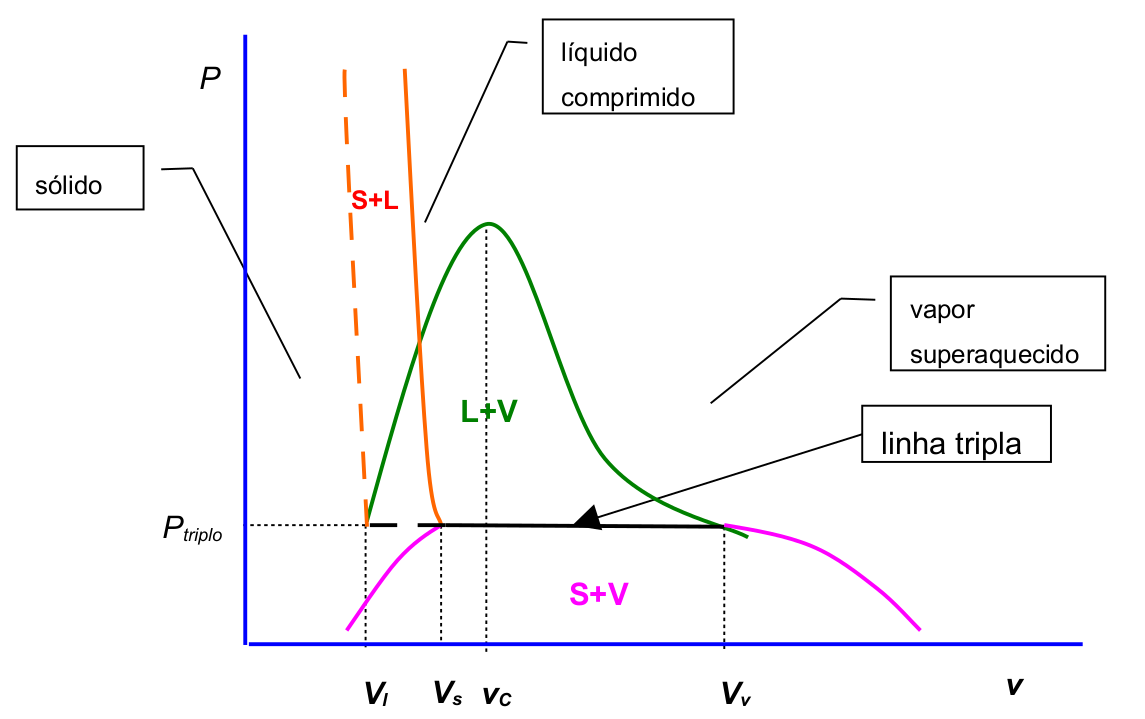
\includegraphics[
            width=0.90\textwidth
        ]   {diagramSolidLiquidVaporWater.png}

        \label{fig:diagramSolidLiquidVaporWater}
    \end{figure}

    \begin{figure}[!htb]
        \caption{%
            Comportamento no plano \gls{pressure}-\gls{temperature} das demais
            substancias
        }

        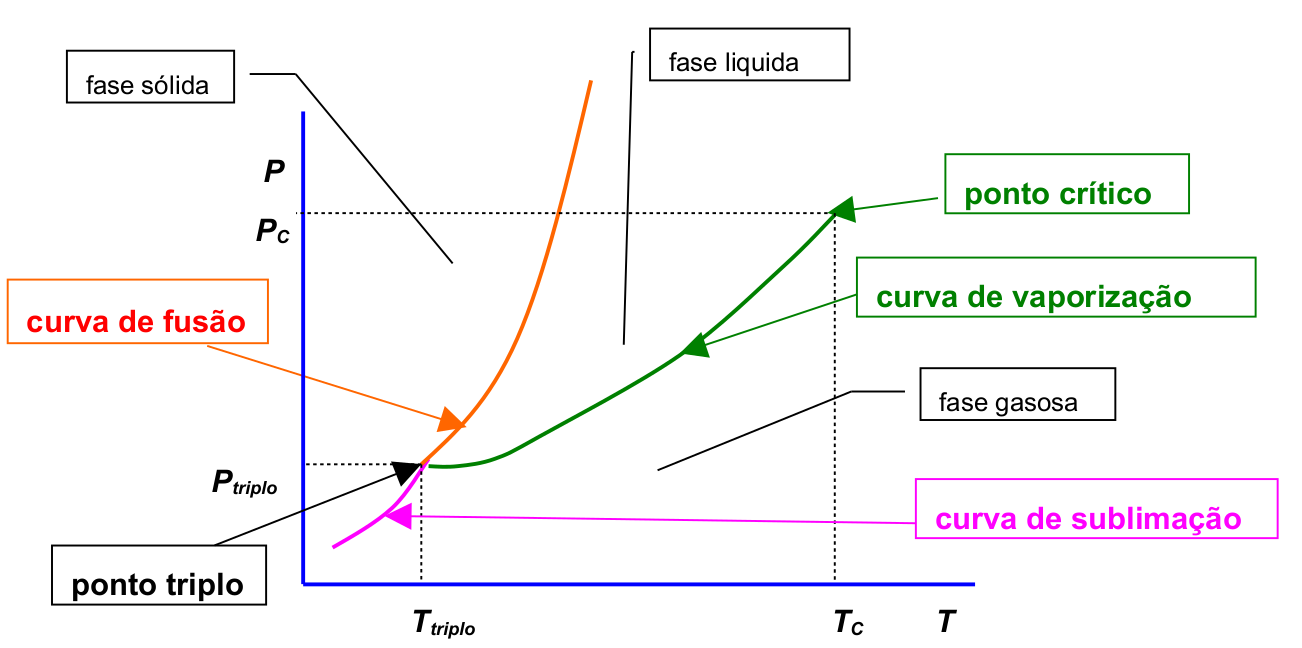
\includegraphics[
            width=0.70\textwidth
        ]   {diagramPTOtherSubstances.png}

        \label{fig:diagramPTOtherSubstances}
    \end{figure}

    \begin{figure}[!htb]
        \caption{%
            Saturação sólido-líquido-vapor para as demais substancias no plano
            \gls{pressure}-\gls{specificVolume}
        }

        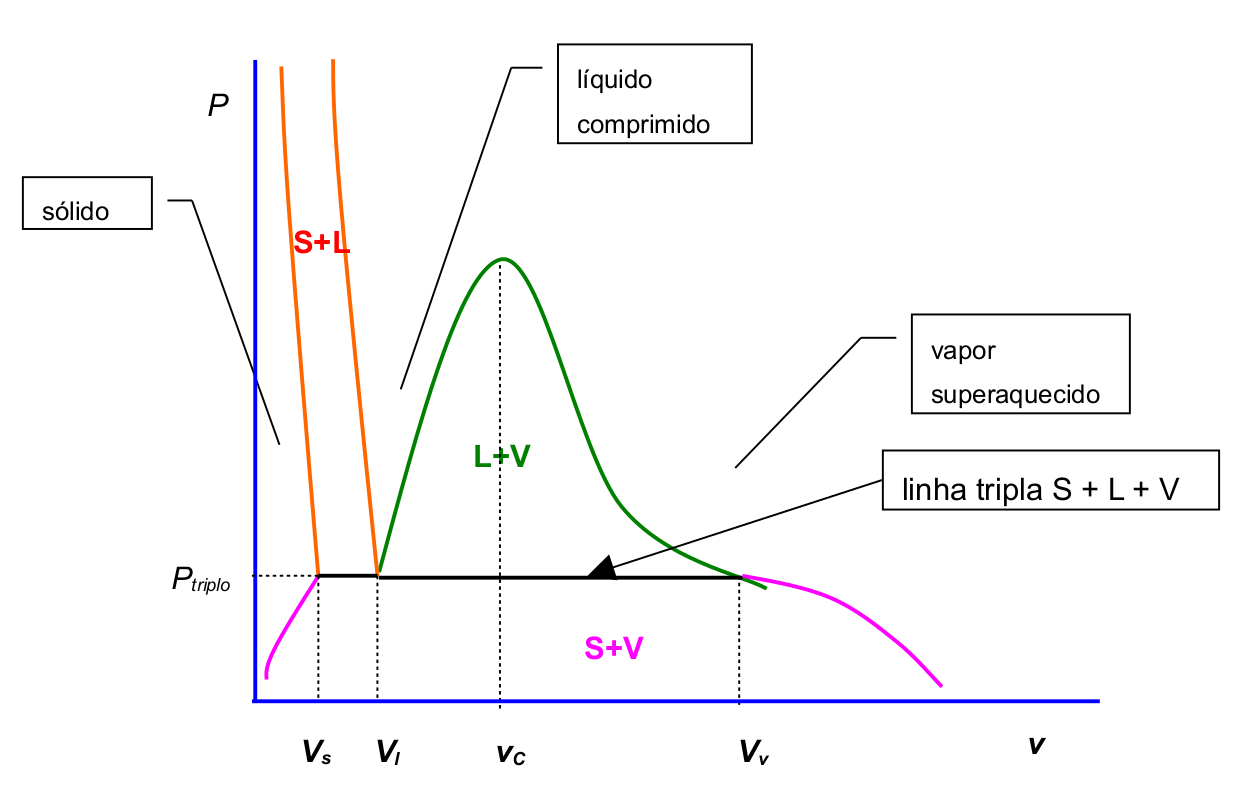
\includegraphics[
            width=0.90\textwidth
        ]   {diagramSolidLiquidVaporOtherSubstances.png}

        \label{fig:diagramSolidLiquidVaporOtherSubstances}
    \end{figure}

    Como seria a visão em escala das projeções
    \gls{temperature},\gls{specificVolume}, \gls{pressure},\gls{specificVolume}
    e \gls{pressure},\gls{temperature} para a água? Veja na
    \cref{fig:diagramRealWater},  como um resultado do programa com
    \command{LK\_proptermo} no notebook curva\_Tv\_Pv\_PT\_agua.ipynb. Observe como foram
    utilizadas as escalas logarítmicas para o volume especifico e para a
    pressão. Com isso, a curva de pressão de vapor ficou com a curvatura
    invertida. Quanto ao programa, você terá a oportunidade de aprender muito
    mais sobre a determinação das propriedades termodinâmicas, inclusive pelo
    pacote \command{LK\_proptermo} e outros, ao longo do texto. Então, você poderá
    determinar com facilidade o valor das propriedades termodinâmicas de
    centenas de substâncias puras!

    \begin{figure}[!htb]
        \caption{%
            Curvas \gls{temperature},\gls{specificVolume},
            \gls{pressure},\gls{specificVolume} e
            \gls{pressure},\gls{temperature}  para a água pura obtidas através
            do programa do autor curva\_Tv\_Pv\_PT\_agua.ipynb
        }

        \begin{subfigure}[b]{0.49\textwidth}
            \caption{}
            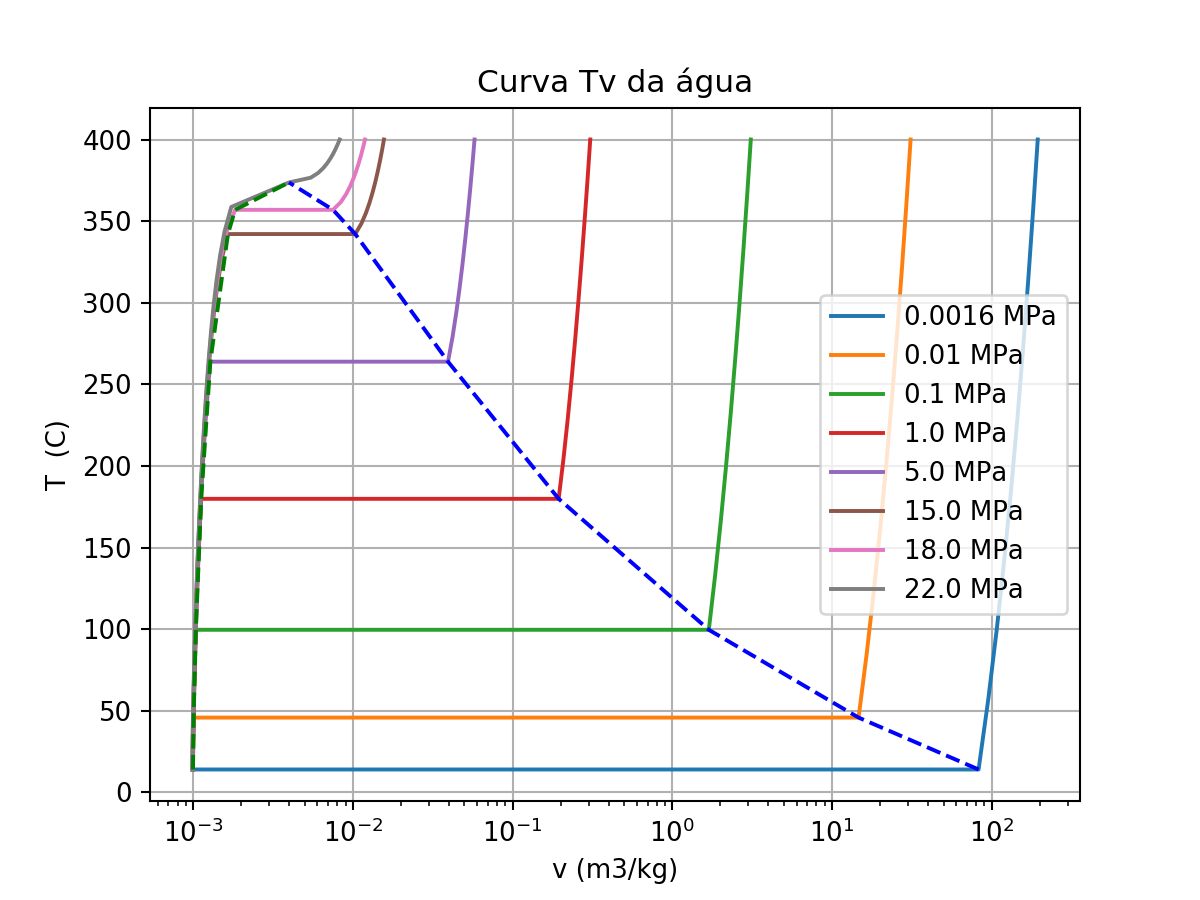
\includegraphics[
                width=\linewidth
            ]  {diagramTvWaterReal.png}
        \end{subfigure}
        %
        \begin{subfigure}[b]{0.49\textwidth}
            \caption{}
            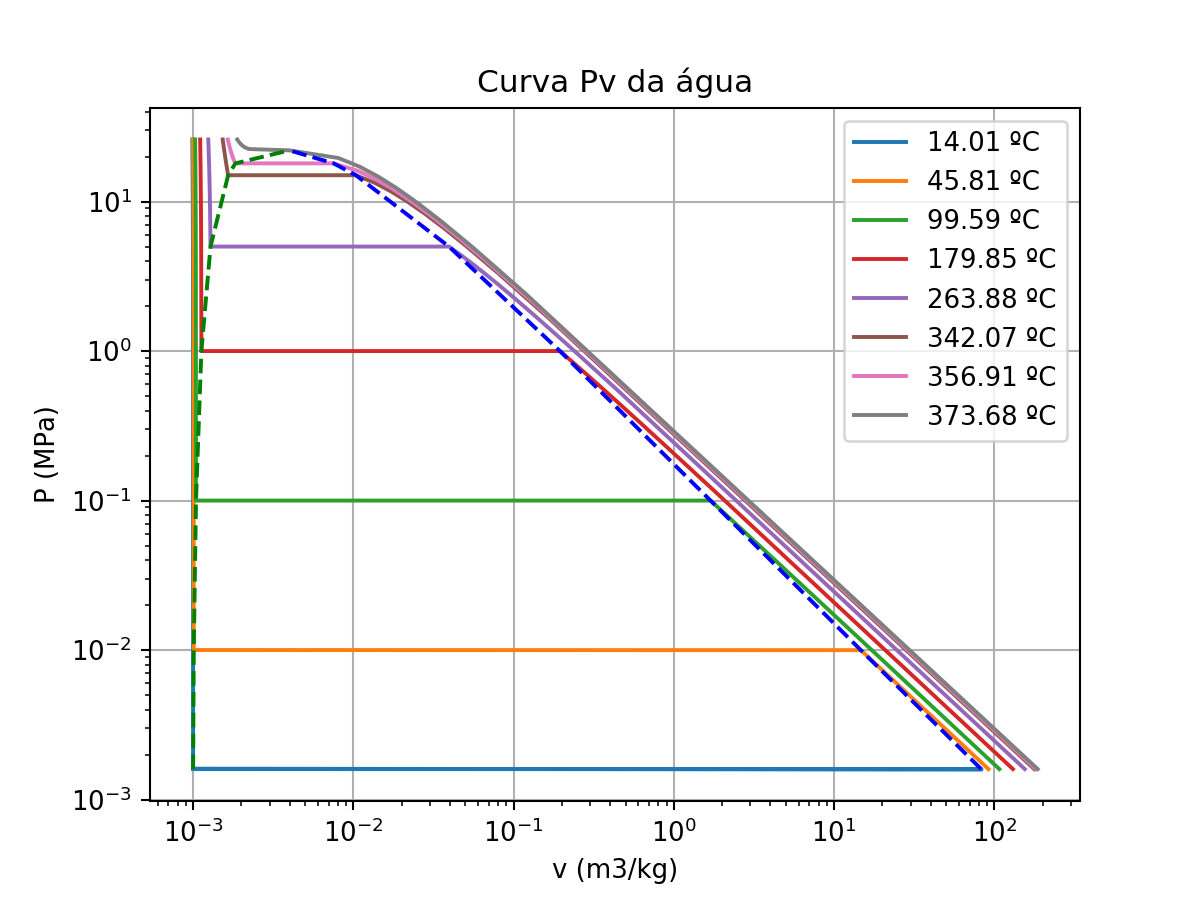
\includegraphics[
                width=\linewidth
            ]   {diagramPvWaterReal.png}
        \end{subfigure}
        %
        \begin{subfigure}[b]{0.49\textwidth}
            \caption{}
            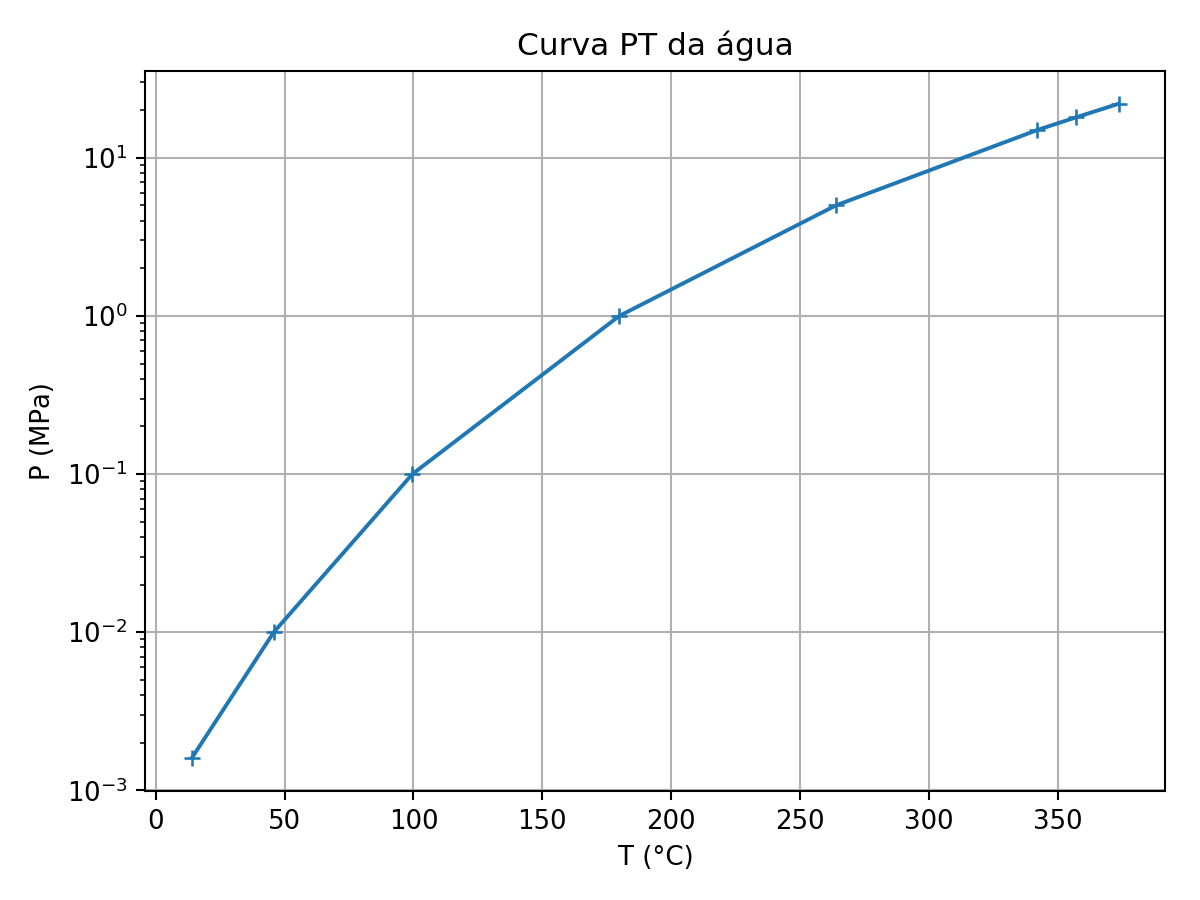
\includegraphics[%
                width=\linewidth
            ]   {diagramPTWaterReal.png}
        \end{subfigure}
        \label{fig:diagramRealWater}
    \end{figure}


    \subsection{O Gás Perfeito}

    A região de gás perfeito (ou ideal) é aquela na fase gasosa em que as
    partículas (átomos, moléculas) se encontram tão afastadas umas das outras
    que praticamente não interagem entre si, ou seja, as forças
    intermoleculares são desprezíveis. Nessas condições, o volume ocupado pelo
    gás será dado pelo volume do recipiente e a pressão que o gás exerce será
    dada unicamente pela colisão das partículas com as paredes.  Podemos então
    escrever, pela Lei de Clapeyron
	%
	\begin{equation} \label{eq:1.4}
        \gls{pressure}
        \gls{volume}
        =
        \gls{mass}
        \gls{gasConstant}
        \gls{temperature}
    \end{equation}

    ou
	%
	\begin{equation}
        \gls{pressure}
        \gls{specificVolume}
        =
        \gls{gasConstant}
        \gls{temperature}\,,
    \end{equation}

    onde \gls{gasConstant} é a constante específica de cada gás. Podemos
    expressar ainda na forma molar
	%
	\begin{equation} \label{eq:1.5}
        \gls{pressure}
        \gls{volume}
        =
        \gls{numberMoles}
        \gls{universalGasConstant}
        \gls{temperature}
    \end{equation}
    %
    ou
    %	%
	\begin{equation}
        \gls{pressure}
        \molar{\gls{specificVolume}}
        =
        \gls{universalGasConstant}
        \gls{temperature}\,,
    \end{equation}

    onde \gls{universalGasConstant} é a constante universal dos gases, cujo
    valor é  \SI{8.31451}{\kilo\joule\per\kilo\mol\per\kelvin} em unidades do
    \gls{si}.

    O que é a forma molar? O número de moles \gls{numberMoles} está relacionado
    com o fato de que um dado volume de qualquer substância pura nas mesmas
    condições de temperatura e pressão contém o mesmo número de moléculas. O
    mol de qualquer coisa (lápis, grãos de arroz, moléculas...) é definido como
    a quantidade de matéria que corresponde ao número de \num{6.022e23} para
    qualquer coisa (lápis, grãos de arroz, moléculas), conhecido como o
    \emph{número de Avogadro}. Devido aos diferentes átomos, a massa que
    corresponde ao mol depende da massa molecular desta substância. A massa
    molecular, por sua vez, é obtida a partir da massa atômica dos
    constituintes da composição química da substância e é  calculada a partir
    da comparação com 1/12 do isótopo 12 do carbono. De qualquer modo, a massa
    molecular (\gls{molecularMass}) de todas as substâncias puras está
    devidamente tabelada (por que os valores de massas moleculares não fornecem
    valores redondos?). Podemos, então, estabelecer as relações entre o número
    de moles \gsub{numberMoles}{substance}, a massa \gsub{mass}{substance} e a
    massa molecular \gsub{molecularMass}{substance}, bem como entre a constante
    universal dos gases perfeitos \gls{universalGasConstant} e a constante
    particular do gás perfeito \gsub{gasConstant}{substance} para a substância
    pura \gls{substance}:
	%
	\begin{equation} \label{eq:1.6}
       \gsub{numberMoles}{substance}
       =
       \gsub{mass}{substance}
       \gsub{molecularMass}{substance}
    \end{equation}

    e, logo
	%
	\begin{equation} \label{eq:gasConstant}
       \gsub{gasConstant}{substance}
       =
       \gls{universalGasConstant}
       \gsub{molecularMass}{substance}\,.
    \end{equation}

    O número de moles não passa de uma forma de representar a massa, mas devido
    a sua conveniência é largamente utilizado. Lembra-se da massa como fator de
    escala? Pois é, exatamente o mesmo princípio se aplica a respeito do número
    de moles. Um cuidado, porém: a massa sempre é conservada, mas o número de
    moles só se conserva se não houverem reações químicas envolvidas.

    Por outro lado, se você tiver dúvidas sobre se deve dividir ou multiplicar
    pela massa molecular \gls{molecularMass}, basta recordar-se que os valores
    molares são sempre maiores do que os seus correspondentes em massa (por
    quê?).

    Lembre-se que a massa molecular é tomada em unidades de massa, tais como o
    grama, o quilograma, a libra-massa. O mol, por sua vez, assume a mesma
    unidade da massa. Por exemplo, a massa molecular (\gls{molecularMass}) do
    metano \ch{CH4} é \num{16.043}, ou seja, para \gls{mass} em gramas,
    \num{16.043} gramas por grama-mol, para \gls{mass} em \si{\kilo\gram},
    \num{16.043} quilogramas por kg-mol, para \gls{mass} em libras-massa,
    \num{16.043} libras-massa por lb-mol, de modo que o número correspondente à
    massa molecular é sempre o mesmo, não importando a unidade de massa
    envolvida. Neste texto nós usaremos o \si{\kilo\mol} (kg-mol) e, portanto,
    associado com a massa em \si{\kilo\gram}. A propósito, o valor da constante
    do gás para o metano é \SI{0.5182446}{\kilo\joule\per\kilo\gram\per\kelvin}
    (ou \si{\joule\per\gram\per\kelvin}). Estes valores também se encontram
    usualmente tabelados ou podem ser simplesmente obtidos, dividindo-se a
    constante universal dos gases  \gls{universalGasConstant} pela massa
    molecular \gls{molecularMass}.

    Na verdade, exceto para os estados incompressíveis, a equação dos gases
    perfeitos é provavelmente uma das mais simples equações de estado (que
    relacionam \gls{pressure}, \gls{specificVolume}, \gls{temperature}). Para
    os líquidos e sólidos, quando puderem ser considerados incompressíveis, a
    equação de estado torna-se $\gls{specificVolume} =$ constante.

    Com frequência precisaremos determinar o valor de
    $\int\gls{pressure}\diff{\gls{volume}}$ sob diversas
    circunstâncias. Então, qual seria o valor daquela integral para um caminho
    isotérmico, isobárico e politrópico, considerando-se o gás como perfeito? E
    para um fluido incompressível? Você acha que a integral de
    \gls{pressure}\diff{\gls{volume}} é uma propriedade termodinâmica?


    \subsection{Comportamento dos Gases Reais}

    De modo geral, para uma região em que a substância pura não se comporta
    como gás perfeito, temos que $\gls{pressure}\gls{specificVolume} \neq
    \gls{gasConstant}\gls{temperature}$. Vamos, então, definir a propriedade
    termodinâmica fator de compressibilidade, \gls{compressibilityFactor}, que
    representa a relação entre o volume específico real \gls{specificVolume}
    (ou \molar{\gls{specificVolume}} e o volume específico que a substância
    exibiria se fosse gás perfeito a \gls{temperature} e \gls{pressure}. Dessa
    forma,
	%
	\begin{equation} \label{eq:1.7}
        \gls{compressibilityFactor}
        =
        \frac{
            \molar{\gls{specificVolume}}
            \functionOf{
                \gls{temperature},
                \gls{pressure}
            }
        }{
            \molar{\gls{specificVolume}}^{*}
            \functionOf{
                \gls{temperature},
                \gls{pressure}
            }
        }
        =
        \frac{
            \molar{\gls{specificVolume}}
            \functionOf{
                \gls{temperature},
                \gls{pressure}
            }
        }{
            \frac{
                \gls{universalGasConstant}
                \gls{temperature}
            }{
                \gls{pressure}
            }
        }
        =
        \frac{
            \gls{pressure}
            \molar{\gls{specificVolume}}
        }{
            \gls{universalGasConstant}
            \gls{temperature}
        }
    \end{equation}
    %
    ou
    %
    \begin{equation} \label{eq:compressibilityFactorDefinition}
        \gls{compressibilityFactor}
        =
        \frac{
           \gls{pressure}
           \gls{specificVolume}
        }{
           \gls{gasConstant}
           \gls{temperature}
        }
    \end{equation}

    Claramente,  $\underset{\gls{pressure} \rightarrow
    0}{\lim}{\gls{compressibilityFactor}} = 1$ , ou seja, a definição de
    \gls{compressibilityFactor} coincide com a equação do gás perfeito quando a
    pressão do gás ou vapor se torna muito menor do que a pressão crítica. Para
    as demais regiões não saturadas, o fator de compressibilidade é uma
    propriedade como outra qualquer e podemos escrever a relação funcional na
    forma das \cref{eq:1.8}.  O que você pode dizer a respeito do fator de
    compressibilidade na região de saturação?
	%
	\begin{equation} \label{eq:1.8}
        \gls{compressibilityFactor}
        =
        \gls{compressibilityFactor}
        \functionOf{
            \gls{temperature},
            \gls{pressure}
        }
        =
        \gls{compressibilityFactor}
        \functionOf{
            \gls{pressure},
            \gls{specificVolume}
        }
        =
        \gls{compressibilityFactor}
        \functionOf{
            \gls{temperature},
            \gls{specificVolume}
        }
    \end{equation}

    As \cref{eq:1.8} não deixam de serem equações de estado, pois se obtivermos
    alguma informação sobre o fator de compressibilidade
    \gls{compressibilityFactor} em função das propriedades mensuráveis
    independentes, p.ex., \gls{temperature}, \gls{pressure}, poderemos
    substituir de volta na equação de definição de \gls{compressibilityFactor},
    \cref{eq:compressibilityFactorDefinition} e então obter a propriedade
    remanescente, no caso \gls{specificVolume}\functionOf{\gls{temperature},
    \gls{pressure}}. Você deve notar que, para os líquidos,
    \gls{compressibilityFactor} é um valor muito menor do que 1 (por quê?) ao
    passo que para os gases longe do ponto crítico, o valor de
    \gls{compressibilityFactor} será geralmente um pouco menor ou um pouco
    maior do que 1. Você sabe dizer o que acontece com o valor de
    \gls{compressibilityFactor} no ponto crítico, ou seja
    \gsub{compressibilityFactor}{critical}?

    Conclusões retiradas de observações experimentais de valores de
    \gls{pressure}, \gls{specificVolume}, \gls{temperature} ou de resultados
    teóricos obtidos da mecânica estatística indicam que o fator de
    compressibilidade pode ser aproximado por uma série infinita de
    $\dfrac{1}{\molar{\gls{specificVolume}}}$ onde os coeficientes da expansão
    são funções apenas da temperatura, da seguinte forma:
	%
	\begin{equation}  \label{eq:1.9}
        \gls{compressibilityFactor}
        \functionOf{
            \gls{temperature},
            \molar{\gls{specificVolume}}
        }
        =
        1
        +
        \frac{
            B\functionOf{\gls{temperature}}
        }{
            \molar{\gls{specificVolume}}
        }
        +
        \frac{
            C\functionOf{\gls{temperature}}
        }{
            \molar{\gls{specificVolume}}^2
        }
        +
        \frac{
            D\functionOf{\gls{temperature}}
        }{
            \molar{\gls{specificVolume}}^3
        }
        +
        \dots\,,
    \end{equation}

    \noindent uma das formas da conhecida equação do virial. A equação de Van
    der Waals (de 1873), uma alteração da equação do gás perfeito, é definida
    pela \cref{eq:1.10}. A equação de Van der Waals é um exemplo de uma equação
    de estado cúbica em \molar{\gls{specificVolume}}.
	%
	\begin{equation} \label{eq:1.10}
        \gls{pressure}
        \functionOf{
            \gls{temperature},
            \molar{\gls{specificVolume}}
        }
        =
        \frac{
            \gls{universalGasConstant}
            \gls{temperature}
        }{
            \molar{\gls{specificVolume}}
            -
            b
        }
        -
        \frac{
            a
        }{
            \molar{\gls{specificVolume}}^2
        }\,,
    \end{equation}
    %
    com as constantes
    %
    \begin{equation} \label{eq:1.11}
        a
        =
        \frac{27}{64}
        \frac{
            \gls{universalGasConstant}^2
            \gsub{temperature}{critical}^2
        }{
            \gsub{pressure}{critical}
        }
    \end{equation}
    %
    e
    %
    \begin{equation} \label{eq:1.12}
        b
        =
        \frac{
            \gls{universalGasConstant}
            \gsub{temperature}{critical}
        }{
            8\gsub{pressure}{critical}
        }\,.
    \end{equation}

    A equação de estado de Van der Waals é bastante simples de se utilizar,
    porém pouco acurada. Para a equação de Van der Waals, o fator de
    compressibilidade no ponto crítico \gsub{compressibilityFactor}{critical}
    será dada por (calcule!):
    %
    \begin{equation} \label{eq:1.13}
        \gsub{compressibilityFactor}{critical}
        =
        \frac{
            \gsub{pressure}{critical}
            \molar{\gls{specificVolume}}_{\gls{critical}}
        }{
            \gls{universalGasConstant}
            \gsub{temperature}{critical}
        }
        =
        \frac{3}{8}\,,
    \end{equation}
	%
%
    um resultado que é significativamente maior do que o
    \gsub{compressibilityFactor}{critical} para qualquer substância pura
    conhecida!

    Uma equação de estado quase igualmente simples e, entretanto,
    surpreendentemente precisa, é, sem dúvida, a equação de \gls{rk} de 1949,
    que, em suas variantes, é utilizada até hoje em cálculos de propriedades de
    misturas e equilíbrio de fases:
    %
    \begin{equation} \label{eq:1.14}
        \gls{pressure}
        =
        \frac{
            \gls{universalGasConstant}
            \gls{temperature}
        }{
            \molar{\gls{specificVolume}}
            -
            b
        }
        -
        \frac{
            a
        }{
            \molar{\gls{specificVolume}}
            \left(
                \molar{\gls{specificVolume}}
                +
                b
            \right)
            T^{\frac{1}{2}}
        }\,,
    \end{equation}
    %
    com as constantes
    %
    \begin{equation} \label{eq:1.15}
        a
        =
        \num{0.42478}
        \frac{
            \gls{universalGasConstant}^2
            \gsub{temperature}{critical}^{\frac{3}{2}}
        }{
            \gsub{pressure}{critical}
        }
    \end{equation}
	%
	\begin{equation} \label{eq:1.16}
        b
        =
        \num{0.08664}
        \frac{
            \gls{universalGasConstant}
            \gsub{temperature}{critical}
        }{
            \gsub{pressure}{critical}
        }\,.
    \end{equation}

    Tanto as constantes da equação de Van der Waals, quanto as de
    \glsxtrlong{rk} foram obtidas, sabendo-se que a isotérmica crítica
    \gsub{temperature}{critical} tem um ponto de inflexão no ponto crítico
    $(\gsub{temperature}{critical},\gsub{pressure}{critical})$, tal que a
    primeira e a segunda derivadas são nulas no ponto crítico.

    Muitas outras modificações da equação \gls{rk} foram propostas e utilizadas
    em anos mais recentes, tais como Redlich-Kwong-Soave, Peng-Robinson e
    Peng-Robinson Modificada.

    Na linha alternativa de equações semi-empíricas, foi desenvolvida para
    hidrocarbonetos a equação de \gls{bwr} (1940) contendo oito constantes
    empíricas. Em 1975 surgiu a equação de \gls{lk}, como uma modificação da
    equação \gls{bwr}, contendo 12 constantes empíricas. Adotada como equação
    básica para o programa computacional {\command{LK\_proptermo}}, a equação de
    estado de \glsxtrlong{lk} será objeto de uma discussão mais detalhada no
    presente trabalho.


    \subsection{Regra dos Estados (Quase) Correspondentes}

    Observe que todas as substâncias puras têm um comportamento \gls{pressure},
    \gls{specificVolume}, \gls{temperature} qualitativamente semelhante à
    descrição que fizemos para a água, principalmente na região de vapor e na
    saturação líquido-vapor, muito embora os valores absolutos das propriedades
    para os diversos estados possam diferir enormemente. Se definirmos as
    grandezas adimensionais temperatura reduzida \gsub{temperature}{reduced} e
    pressão reduzida \gsub{pressure}{reduced} em relação ao ponto crítico
    \gsub{temperature}{critical} e \gsub{pressure}{critical} (que, como vimos,
    são únicos para cada substância pura), na forma:
    %	%
	\begin{equation} \label{eq:1.17}
        \gsub{temperature}{reduced}
        =
        \frac{
            \gls{temperature}
        }{
            \gsub{temperature}{critical}
        }
    \end{equation}
    %
    e	%
	\begin{equation}
        \gsub{pressure}{reduced}
        =
        \frac{
            \gls{pressure}
        }{
            \gsub{pressure}{critical}
        }\,,
    \end{equation}
    %
    \noindent então descobriremos que
    \gls{compressibilityFactor}\functionOf{\gsub{pressure}{reduced},
    \gsub{temperature}{reduced}} assumirá (quase) os mesmos valores,
    independentemente da substância pura que estamos considerando. Este
    comportamento aparentemente surpreendente é a chamada \emph{\enquote{Lei}
    ou Regra dos Estados (quase) Correspondentes}.

    Por outro lado, todas as equações de estado podem ser expressas em termos
    de coordenadas reduzidas. Com alguma manipulação, a equação de Van der
    Waals se torna:
	%
	\begin{equation} \label{eq:1.18}
        \gls{compressibilityFactor}^3
        -
        \left(
            \frac{1}{8}
            \gsub{pressure}{reduced}
            \gsub{temperature}{reduced}
            +
            1
        \right)
        \gls{compressibilityFactor}^2
        +
        \left(
            \frac{27}{64}
            \gsub{pressure}{reduced}
            \gsub{temperature}{reduced}^2
        \right)
        \gls{compressibilityFactor}
        -
        \frac{27}{512}
        \gsub{pressure}{reduced}^2
        \gsub{temperature}{reduced}^3
        =
        F
        \functionOf{
            \gls{compressibilityFactor},
            \gsub{pressure}{reduced},
            \gsub{temperature}{reduced}
        }
        =
        0\,.
    \end{equation}

    A equação de estado generalizada de \gls{lk}, com as 12 constantes $b_1,
    b_2, b_3, b_4, c_1, c_2, c_3, c_4, d_1, d_2, \beta, \gamma$, que são
    tabeladas para um fluido de referência e para um fluido simples é definida
    pelo conjunto das Eqs. 1.19-22, da seguinte forma:
	%
	\begin{equation} \label{eq:1.19}
        \gls{compressibilityFactor}
        =
        \frac{
            \gsub{pressure}{reduced}
            \gls{modifiedReducedVolume}
        }{
            \gsub{temperature}{reduced}
        }
        =
        1
        +
        \frac{
            B
        }{
            \gls{modifiedReducedVolume}
        }
        +
        \frac{
            C
        }{
            \gls{modifiedReducedVolume}^2
        }
        +
        \frac{
            D
        }{
            \gls{modifiedReducedVolume}^3
        }
        +
        \frac{
            c_4
        }{
            \gsub{temperature}{reduced}^3
            \gls{modifiedReducedVolume}^2
        }
        \left(
            \beta
            +
            \frac{
                \gamma
            }{
                \gls{modifiedReducedVolume}^2
            }
        \right)
        \exp{
            \left(
                -\frac{
                    \gamma
                }{
                    \gls{modifiedReducedVolume}^2
                }
            \right)
        }
    \end{equation}
	%
	\begin{equation} \label{eq:1.20}
        B
        =
        b_1
        -
        \frac{
            b_2
        }{
            \gsub{temperature}{reduced}
        }
        -
        \frac{
            b_3
        }{
            \gsub{temperature}{reduced}^2
        }
        -
        \frac{
            b_4
        }{
            \gsub{temperature}{reduced}^3
        }
    \end{equation}
	%
	\begin{equation} \label{eq:1.21}
        C
        =
        c_1
        -
        \frac{
            c_2
        }{
            \gsub{temperature}{reduced}
        }
        +
        \frac{
            c_3
        }{
            \gsub{temperature}{reduced}^3
        }
    \end{equation}
	%
	\begin{equation} \label{eq:1.22}
        D
        =
        d_1
        +
        \frac{
            d_2
        }{
            \gsub{temperature}{reduced}
        }
    \end{equation}

    onde a conveniente definição de \gls{modifiedReducedVolume} é:
	%
	\begin{equation} \label{eq:1.23}
        \gls{modifiedReducedVolume}
        =
        \frac{
            \gls{specificVolume}
        }{
            \frac{
                \gls{gasConstant}
                \gsub{temperature}{critical}
            }{
                \gsub{pressure}{critical}
            }
        }
        \neq
        \gsub{specificVolume}{reduced}
    \end{equation}

    Observe que aqui o volume específico reduzido é \gls{modifiedReducedVolume}
    ao invés de $\gsub{specificVolume}{reduced} =
    \dfrac{\gls{specificVolume}}{\gsub{specificVolume}{critical}}$, pois é
    difícil obter-se o valor do volume crítico \gsub{specificVolume}{critical}
    experimentalmente.

    Qual é a razão de se denominar de lei dos estados \enquote{quase}
    correspondentes? Embora qualitativamente semelhante, verifica-se que o
    valor de
    \gls{compressibilityFactor}\functionOf{\gsub{temperature}{reduced},
    \gsub{pressure}{reduced}} não é exatamente o mesmo para quaisquer
    substâncias puras. Pense um pouco: Se os estados fossem exatamente
    correspondentes, qual seria o gráfico esperado para a curva de pressão de
    vapor de qualquer substância pura em coordenadas reduzidas
    \gsub{pressure}{reduced},\gsub{temperature}{reduced}?

    Veja a \cref{fig:waterNondimensionalVaporPressureCurves}, na qual foram,
    com \command{LK\_proptermo}, computacionalmente obtidas e plotadas as curvas de
    pressão de vapor das substâncias puras \ch{He}, \ch{H2}, \ch{Ar}, \ch{CH4},
    \ch{N2}, \ch{C3H8}, \ch{NH3}, \ch{H2O} e \ch{C2H5OH} na forma adimensional
    $\log_{10}(\gsub{pressure}{reduced})$ em função de
    $\frac{1}{\gsub{temperature}{reduced}}$. Observe que cada substância pura
    tem a sua própria curva de pressão de vapor mesmo em coordenadas reduzidas
    e que com essas variáveis, as curvas são quase retas.  Pode dizer por que
    elas são quase retas?


    \subsection{O Fator Acêntrico de Pitzer}

    Entre as muitas possibilidades de se aperfeiçoar o modelo generalizado, uma
    delas se tornou muito popular: o uso, além de \gsub{temperature}{reduced} e
    \gsub{pressure}{reduced}, do fator acêntrico de Pitzer,
    \gls{PitzerAcentricFactor}, como um terceiro parâmetro para se definir
    \gls{compressibilityFactor}, utilizando-se a seguinte forma linear de
    correção:
    %
    \begin{equation} \label{eq:1.24}
        \gls{compressibilityFactor}
        \functionOf{
            \gsub{temperature}{reduced},
            \gsub{pressure}{reduced},
            \gls{PitzerAcentricFactor}
        }
        =
        \state{\gls{compressibilityFactor}}{0}
        \functionOf{
            \gsub{temperature}{reduced},
            \gsub{pressure}{reduced}
        }
        +
        \gls{PitzerAcentricFactor}
        \state{\gls{compressibilityFactor}}{1}
        \functionOf{
            \gsub{temperature}{reduced},
            \gsub{pressure}{reduced}
        }\,.
    \end{equation}

    Os valores de \state{\gls{compressibilityFactor}}{0} são aqueles obtidos com a
    aplicação direta de \gls{lk} e seus resultados se aplicam muito bem para os
    chamados fluidos simples, por exemplo \ch{Xe}, \ch{Ra}, \ch{Ar} e \ch{CH4},
    cujas moléculas são não-polares e mantêm simetria esférica. Os valores de
    correção \state{\gls{compressibilityFactor}}{1}, por sua vez, só dependem de
    \gsub{temperature}{reduced},\gsub{pressure}{reduced}.

    Por outro lado, note na \cref{fig:waterNondimensionalVaporPressureCurves}
    que para os fluidos simples o valor da pressão reduzida de saturação
    \gsub{satPressure}{reduced}\functionOf{\gsub{temperature}{reduced}} para
    $\gsub{temperature}{reduced} = \num{0.7}$ é igual a \num{0.1} e que, além
    disso, este valor é diferente para cada uma das demais substância puras.
    Definiu-se então o fator acêntrico de Pitzer com a ajuda da \cref{eq:1.25}
    tal que no caso dos fluidos simples resultasse em
    $\gls{PitzerAcentricFactor} = 0$ (por quê?).

    \begin{figure}[!htb]
        \caption{%
            Curvas de pressão de vapor adimensionais para diversas substâncias
            puras calculadas computacionalmente e seus respectivos valores do
            fator acêntrico de Pitzer \gls{PitzerAcentricFactor}.
        }
        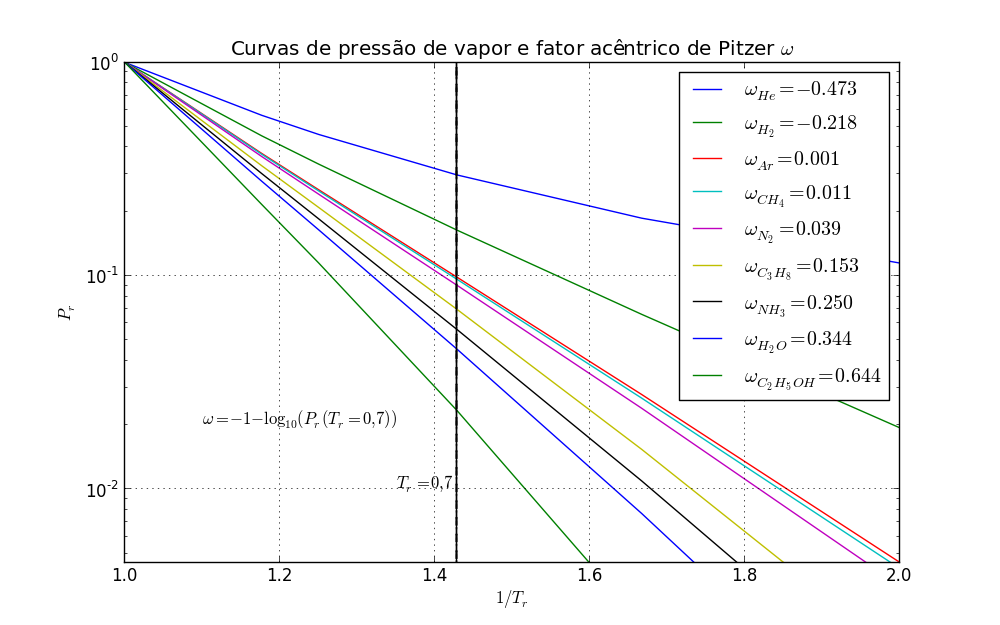
\includegraphics[%
            width=0.75\textwidth
        ]   {waterNondimensionalVaporPressureCurves.png}

        \label{fig:waterNondimensionalVaporPressureCurves}
    \end{figure}
	%
	\begin{equation} \label{eq:1.25}
        \gls{PitzerAcentricFactor}
        =
        -1
        -
        \log_{10}{
            \left[
                \gsub{satPressure}{reduced}
                \functionOf{
                    \gsub{temperature}{reduced} = \num{0.7}
                }
            \right]
        }
    \end{equation}

    Verifique a interseção da linha de $\gsub{temperature}{reduced} =
    \num{0.7}$ para a obtenção do valor de \gls{PitzerAcentricFactor} para cada
    uma das substâncias puras. Na legenda da figura estão registrados os
    valores de \gls{PitzerAcentricFactor}, do menor ao maior, para cada uma
    delas. Na verdade, existem na literatura tabelas de
    \gls{PitzerAcentricFactor} para as substâncias puras, bem como tabelas e
    programas de computador para as correções \state{\gls{compressibilityFactor}}{1}
    bem como para as demais correções. Com o apoio desses programas, seu uso
    não é tão complicado quanto possa parecer. Um desses programas,
    \command{LK\_proptermo}, bem como suas aplicações, será estudado detalhadamente e
    extensivamente utilizado.

    Os diagramas generalizados com as correções do fator acêntrico também
    produzem bons resultados na região de saturação das substâncias puras, para
    as moléculas não-polares. Voltemos ao metano: qual seria a pressão de
    saturação correspondente a \SI{-110}{\celsius}? Pelos diagramas
    generalizados e computacionalmente, obtemos $\gls{satPressure} =
    \SI{1.7896}{\mega\pascal}$ e pelas tabelas do metano saturado,
    $\gls{satPressure} = \SI{1.803}{\mega\pascal}$, o que dá cerca de
    \SI{0.7}{\percent} de diferença! A propósito, podemos agora perceber da
    figura porque os resultados para o metano no nosso exemplo foram tão
    próximos dos valores das tabelas: \gls{PitzerAcentricFactor} do metano é
    igual a \num{0.011}, com a sua curva de vapor muito próxima do argônio,
    cujo \gls{PitzerAcentricFactor} é igual a \num{0.001} e, portanto, tornando
    o um exemplo razoável de substância simples....

    Na região de saturação, onde \gls{vaporQuality} é o título do vapor,
    podemos escrever (você já demonstrou isso antes...):
    %
    \begin{subequations} \label{eq:1.26}
        \begin{equation}
            \gls{compressibilityFactor}
            \functionOf{
                \gsub{pressure}{reduced},
                \gls{vaporQuality},
                \gls{PitzerAcentricFactor}
            }
            =
            \left(
                1 - \gls{vaporQuality}
            \right)
            \gsub{compressibilityFactor}{liquid}
            \functionOf{
                \gsub{pressure}{reduced},
                \gls{PitzerAcentricFactor}
            }
            +
            \gls{vaporQuality}
            \gsub{compressibilityFactor}{vapor}
            \functionOf{
                \gsub{pressure}{reduced},
                \gls{PitzerAcentricFactor}
            }
        \end{equation}
        %
        \begin{equation}
            \gls{compressibilityFactor}
            \functionOf{
                \gsub{temperature}{reduced},
                \gls{vaporQuality},
                \gls{PitzerAcentricFactor}
            }
            =
            \left(
                1 - \gls{vaporQuality}
            \right)
            \gsub{compressibilityFactor}{liquid}
            \functionOf{
                \gsub{temperature}{reduced},
                \gls{PitzerAcentricFactor}
            }
            +
            \gls{vaporQuality}
            \gsub{compressibilityFactor}{vapor}
            \functionOf{
                \gsub{temperature}{reduced},
                \gls{PitzerAcentricFactor}
            }\,,
        \end{equation}
    \end{subequations}
    %
    onde cada um dos termos em \gls{compressibilityFactor} sofre o efeito do
    fator acêntrico \gls{PitzerAcentricFactor}, da mesma forma que já foi
    exposto anteriormente.

    \subsection{%
        As moléculas polares e a correção com o fator de polaridade de Wu e
        Stiel
    }

    Embora com a correção a três parâmetros \gsub{temperature}{reduced},
    \gsub{pressure}{reduced} e \gls{PitzerAcentricFactor} se obtenham
    resultados adequados para substâncias puras não-polares ou até mesmo
    fracamente polares, para substâncias puras fortemente polares, como
    \ch{H2O} ou \ch{NH3}, os erros podem ser muito significativos. Surgiu,
    então, a necessidade de se usar algum parâmetro adicional para representar
    o efeito da polaridade.  Dentre as várias possibilidades da literatura,
    escolhemos o parâmetro denominado fator de polaridade \gls{WuPolarFactor}
    de Wu-Stiel.  Estendendo então a correção linear de Pitzer, pode-se
    aplicá-lo da seguinte forma:
	%
	\begin{equation} \label{eq:1.27}
        \gls{compressibilityFactor}
        \functionOf{
            \gsub{temperature}{reduced},
            \gsub{pressure}{reduced},
            \gls{PitzerAcentricFactor},
            \gls{WuPolarFactor}
        }
        =
        \state{\gls{compressibilityFactor}}{0}
        \functionOf{
            \gsub{temperature}{reduced},
            \gsub{pressure}{reduced}
        }
        +
        \gls{PitzerAcentricFactor}
        \state{\gls{compressibilityFactor}}{1}
        \functionOf{
            \gsub{temperature}{reduced},
            \gsub{pressure}{reduced}
        }
        +
        \gls{WuPolarFactor}
        \state{\gls{compressibilityFactor}}{2}
        \functionOf{
            \gsub{temperature}{reduced},
            \gsub{pressure}{reduced}
        }
        \,.
    \end{equation}

    O fator \gls{WuPolarFactor} é definido a partir do volume molar do líquido
    saturado a $\gsub{temperature}{reduced} = \num{0.8}$, de forma que
    $\gls{WuPolarFactor} = \num{1.0}$ para a água, $\gls{WuPolarFactor} = 0$
    para as substâncias não-polares e terá valores intermediários para as
    demais substâncias. Nessa abordagem, a água é usada como referência e para
    a obtenção das propriedades da água é empregada a equação de estado de
    Keenan. Os valores de \gls{WuPolarFactor}, por sua vez, devem ser obtidos
    de tabelas.

    O fator de compressibilidade \gls{compressibilityFactor} em função da
    temperatura reduzida \gsub{temperature}{reduced} com
    \gsub{pressure}{reduced} constante não é comumente apresentado na
    literatura. Na \cref{fig:waterCompressibilityFactor} você pode analisar o
    comportamento dessa função, calculada computacionalmente com \command{LK\_proptermo},
    para a água, utilizando-se os valores do fator acêntrico e do fator de
    Wu-Stiel para esta substância pura. Já na
    \cref{fig:propaneCompressibilityFactor}, que se refere ao propano
    \ch{C3H8}, podemos ver que \gls{compressibilityFactor} pode ser maior do
    que \num{1} quando \gsub{temperature}{reduced} é maior do que \num{2}.
    Chamamos ainda a atenção para o comportamento supercrítico do fator de
    compressibilidade.  Observe que para $\gsub{pressure}{reduced} = 10$,
    \gls{compressibilityFactor} alcança valores bastante elevados.

    \begin{figure}[!htb]
        \caption{%
            Curvas  do fator de compressibilidade \gls{compressibilityFactor}
            da água $(\gls{PitzerAcentricFactor} = \num{0.344},
            \gls{WuPolarFactor} = 1)$ em função de temperatura reduzida
            \gsub{temperature}{reduced} tendo como parâmetro o valor de
            \gsub{pressure}{reduced}.
        }

        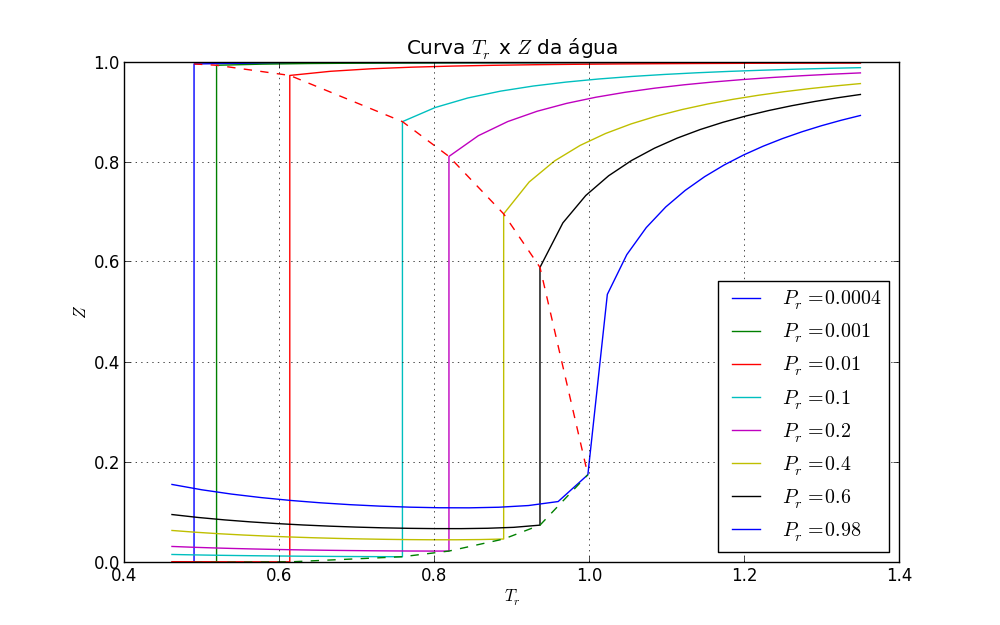
\includegraphics[%
            width=0.85\textwidth
        ]   {waterCompressibilityFactor.png}

        \label{fig:waterCompressibilityFactor}
    \end{figure}

    Para uma visão mais convencional do fator de compressibilidade
    \gls{compressibilityFactor} do propano em função da pressão reduzida
    \gsub{pressure}{reduced}, tendo agora \gsub{temperature}{reduced} como
    parâmetro, veja a \cref{fig:propaneCompressibilityFactorVsPressure}, também
    obtida computacionalmente. Da mesma forma que na
    \cref{fig:propaneCompressibilityFactor}, estude o comportamento do fator de
    compressibilidade em condições supercríticas.  Observe que o fator
    determinante é a pressão.

    \begin{figure}[!htb]
        \caption{%
            Curvas obtidas computacionalmente do fator de
            compressibilidade \gls{compressibilityFactor} do propano
            $(\gls{PitzerAcentricFactor} = \num{0.153}, \gls{WuPolarFactor} =
            0)$ em função da temperatura reduzida \gsub{temperature}{reduced}
            tendo como parâmetro o valor de \gsub{pressure}{reduced}
        }

        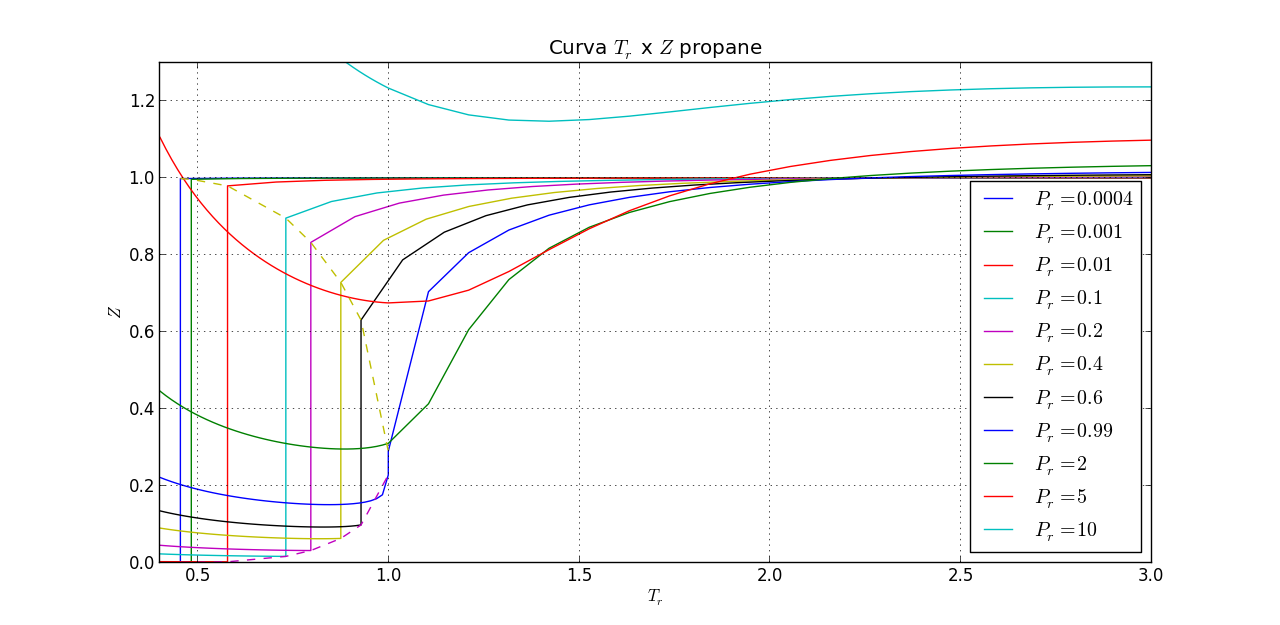
\includegraphics[%
            width=0.85\textwidth
        ]   {propaneCompressibilityFactor.png}

        \label{fig:propaneCompressibilityFactor}
    \end{figure}


    \begin{figure}[!htb]
        \caption{%
            Curvas obtidas computacionalmente do fator de
            compressibilidade \gls{compressibilityFactor} do propano em função
            da pressão reduzida \gsub{pressure}{reduced} tendo como parâmetro o
            valor de \gsub{temperature}{reduced} .
        }

        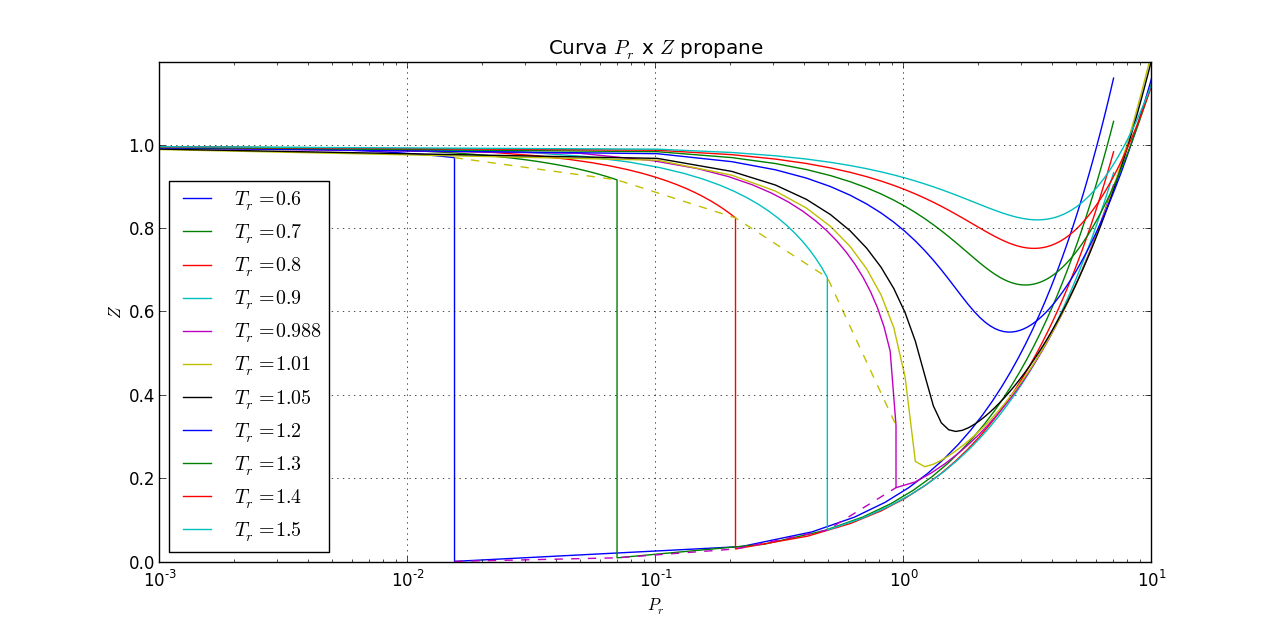
\includegraphics[%
            width=0.85\textwidth
        ]   {propaneCompressibilityFactorVsPressure.png}

        \label{fig:propaneCompressibilityFactorVsPressure}
    \end{figure}


    \subsection{As Propriedades Não Mensuráveis}

    Note que até agora só pudemos nos referenciar às propriedades
    termodinâmicas mensuráveis \gls{pressure}, \gls{temperature},
    \gls{specificVolume}, \gls{vaporQuality} e aprendemos que podemos expressar
    o fator de compressibilidade $\gls{compressibilityFactor} =
    \gls{compressibilityFactor}\functionOf{\gsub{temperature}{reduced},
        \gsub{pressure}{reduced}, \gls{PitzerAcentricFactor},
    \gls{WuPolarFactor}}$ de qualquer substância pura, cuja assinatura é
    $(\gls{molecularMass}, \gsub{temperature}{critical},
    \gsub{pressure}{critical}, \gls{PitzerAcentricFactor},
    \gls{WuPolarFactor})$, onde \gls{molecularMass} é massa molecular e
    portanto, determinamos \gls{specificVolume}\functionOf{\gls{pressure},
    \gls{temperature}}.

    Por outro lado, qual é a origem das propriedades termodinâmicas não
    mensuráveis e como se avaliar o seu valor? Esses tópicos serão objetos de
    discussão nos próximos capítulos, mas antes vamos estabelecer as bases para
    as Leis da Termodinâmica. Veremos que a partir das tais leis, algumas
    propriedades serão convenientemente definidas e a partir dessas muitas
    outras mais, sempre obedecendo ao Postulado dos Estados.

    Descobriremos também que o valor absoluto das propriedades termodinâmicas
    não mensuráveis não tem significado. Finalmente, tenha sempre em mente que,
    quaisquer que sejam as suas origens, as propriedades termodinâmicas não
    dependem de processo algum para sua existência. Uma vez definidas por
    conveniência a partir de um determinado processo, elas se desprendem e
    adquirem, por assim dizer, vida própria!
